\documentclass{standalone}
\usepackage{tikz}
\usetikzlibrary{patterns, positioning}


\begin{document}
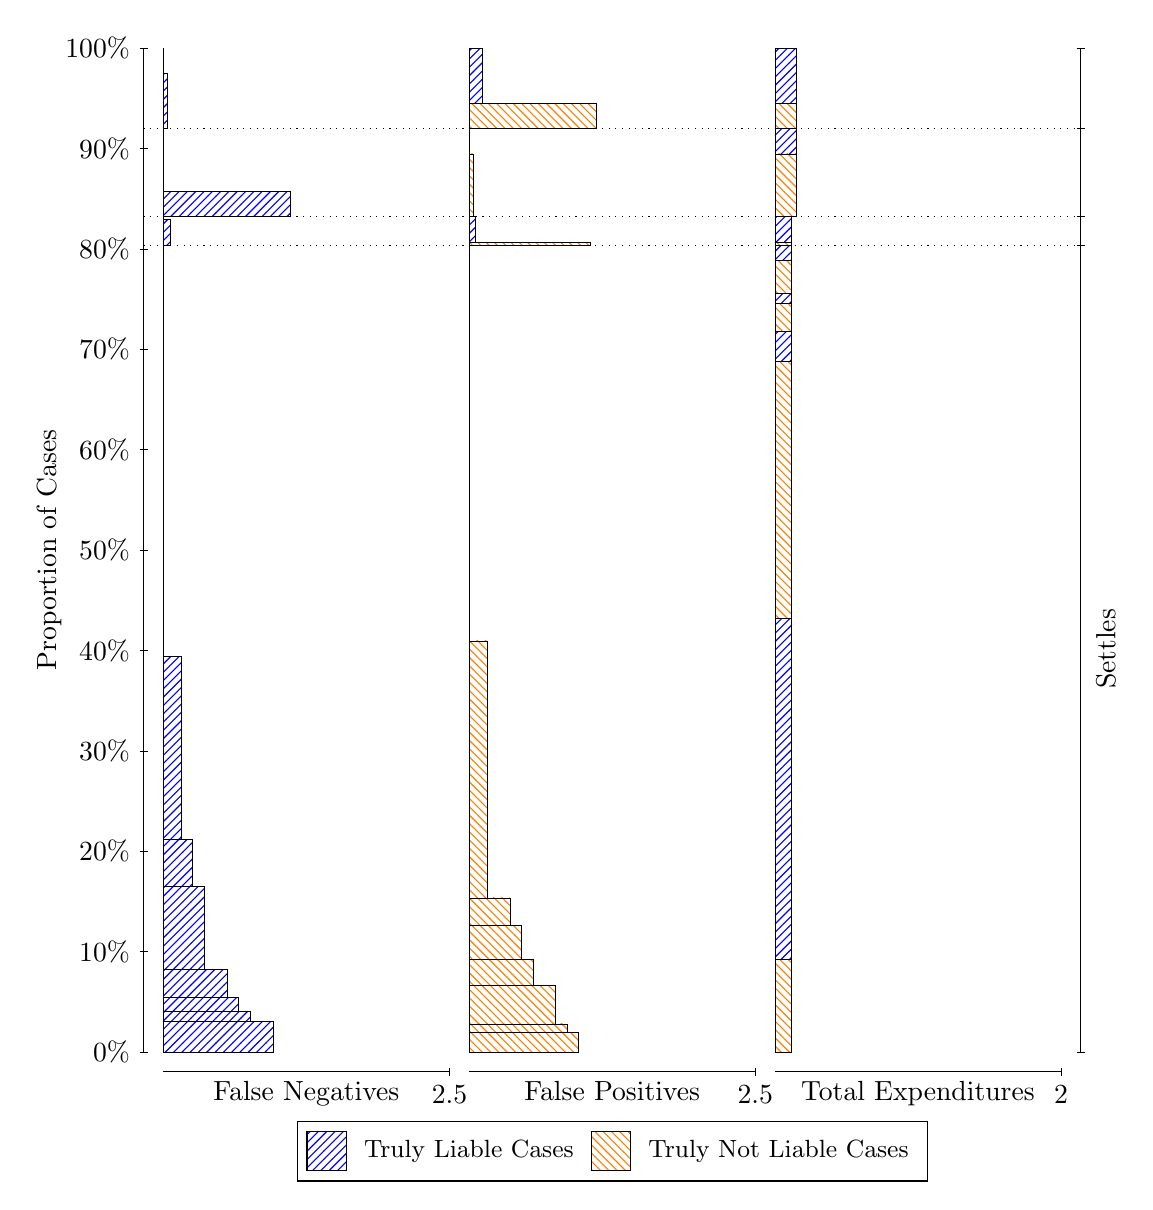
\begin{tikzpicture}
\draw[black, very thin] (1.5,1.75) -- (1.5,14.5);
\node[rotate=90, text=black, anchor=center] at (0.3, 8.125) {Proportion of Cases};
\draw[black, very thin] (1.45,1.75) -- (1.55,1.75);
\node[text=black, anchor=east] at (1.45, 1.75) {0\%};
\draw[black, very thin] (1.45,3.025) -- (1.55,3.025);
\node[text=black, anchor=east] at (1.45, 3.025) {10\%};
\draw[black, very thin] (1.45,4.3) -- (1.55,4.3);
\node[text=black, anchor=east] at (1.45, 4.3) {20\%};
\draw[black, very thin] (1.45,5.575) -- (1.55,5.575);
\node[text=black, anchor=east] at (1.45, 5.575) {30\%};
\draw[black, very thin] (1.45,6.85) -- (1.55,6.85);
\node[text=black, anchor=east] at (1.45, 6.85) {40\%};
\draw[black, very thin] (1.45,8.125) -- (1.55,8.125);
\node[text=black, anchor=east] at (1.45, 8.125) {50\%};
\draw[black, very thin] (1.45,9.4) -- (1.55,9.4);
\node[text=black, anchor=east] at (1.45, 9.4) {60\%};
\draw[black, very thin] (1.45,10.675) -- (1.55,10.675);
\node[text=black, anchor=east] at (1.45, 10.675) {70\%};
\draw[black, very thin] (1.45,11.95) -- (1.55,11.95);
\node[text=black, anchor=east] at (1.45, 11.95) {80\%};
\draw[black, very thin] (1.45,13.225) -- (1.55,13.225);
\node[text=black, anchor=east] at (1.45, 13.225) {90\%};
\draw[black, very thin] (1.45,14.5) -- (1.55,14.5);
\node[text=black, anchor=east] at (1.45, 14.5) {100\%};

\draw[black, very thin] (13.4,1.75) -- (13.4,14.5);
\draw[black, very thin] (13.35,1.75) -- (13.45,1.75);
\node[anchor=west] at (13.35, 1.75) {};
\draw[black, very thin] (13.35,11.989) -- (13.45,11.989);
\node[anchor=west] at (13.35, 11.989) {};
\draw[black, very thin] (13.35,12.362) -- (13.45,12.362);
\node[anchor=west] at (13.35, 12.362) {};
\draw[black, very thin] (13.35,13.477) -- (13.45,13.477);
\node[anchor=west] at (13.35, 13.477) {};
\draw[black, very thin] (13.35,14.5) -- (13.45,14.5);
\node[anchor=west] at (13.35, 14.5) {};

\draw[black, very thin, pattern color=blue, pattern=north east lines] (1.75,1.75) rectangle (3.1398,2.1388);
\draw[black, very thin, pattern color=blue, pattern=north east lines] (1.75,2.1388) rectangle (2.8491,2.262);
\draw[black, very thin, pattern color=blue, pattern=north east lines] (1.75,2.262) rectangle (2.7037,2.4461);
\draw[black, very thin, pattern color=blue, pattern=north east lines] (1.75,2.4461) rectangle (2.5584,2.7971);
\draw[black, very thin, pattern color=blue, pattern=north east lines] (1.75,2.7971) rectangle (2.2678,3.8551);
\draw[black, very thin, pattern color=blue, pattern=north east lines] (1.75,3.8551) rectangle (2.1224,4.4487);
\draw[black, very thin, pattern color=blue, pattern=north east lines] (1.75,4.4487) rectangle (1.9771,6.7694);
\draw[black, very thin, pattern color=orange, pattern=north west lines] (1.75,6.7694) rectangle (1.75,11.989);
\draw[black, very thin, pattern color=blue, pattern=north east lines] (1.75,11.989) rectangle (1.8318,12.321);
\draw[black, very thin, pattern color=orange, pattern=north west lines] (1.75,12.321) rectangle (1.75,12.362);
\draw[black, very thin, pattern color=blue, pattern=north east lines] (1.75,12.362) rectangle (3.3668,12.682);
\draw[black, very thin, pattern color=orange, pattern=north west lines] (1.75,12.682) rectangle (1.75,13.477);
\draw[black, very thin, pattern color=blue, pattern=north east lines] (1.75,13.477) rectangle (1.8045,14.181);
\draw[black, very thin, pattern color=orange, pattern=north west lines] (1.75,14.181) rectangle (1.75,14.5);
\draw[black, very thin, pattern color=orange, pattern=north west lines] (5.6333,1.75) rectangle (7.0231,2.0009);
\draw[black, very thin, pattern color=orange, pattern=north west lines] (5.6333,2.0009) rectangle (6.8777,2.1072);
\draw[black, very thin, pattern color=orange, pattern=north west lines] (5.6333,2.1072) rectangle (6.7324,2.5914);
\draw[black, very thin, pattern color=orange, pattern=north west lines] (5.6333,2.5914) rectangle (6.4417,2.9296);
\draw[black, very thin, pattern color=orange, pattern=north west lines] (5.6333,2.9296) rectangle (6.2964,3.3548);
\draw[black, very thin, pattern color=orange, pattern=north west lines] (5.6333,3.3548) rectangle (6.1511,3.7062);
\draw[black, very thin, pattern color=orange, pattern=north west lines] (5.6333,3.7062) rectangle (5.8604,6.97);
\draw[black, very thin, pattern color=blue, pattern=north east lines] (5.6333,6.97) rectangle (5.6333,11.989);
\draw[black, very thin, pattern color=orange, pattern=north west lines] (5.6333,11.989) rectangle (7.1684,12.031);
\draw[black, very thin, pattern color=blue, pattern=north east lines] (5.6333,12.031) rectangle (5.7151,12.362);
\draw[black, very thin, pattern color=orange, pattern=north west lines] (5.6333,12.362) rectangle (5.6878,13.157);
\draw[black, very thin, pattern color=blue, pattern=north east lines] (5.6333,13.157) rectangle (5.6333,13.477);
\draw[black, very thin, pattern color=orange, pattern=north west lines] (5.6333,13.477) rectangle (7.2502,13.796);
\draw[black, very thin, pattern color=blue, pattern=north east lines] (5.6333,13.796) rectangle (5.7968,14.5);
\draw[black, very thin, pattern color=orange, pattern=north west lines] (9.5167,1.75) rectangle (9.721,2.9296);
\draw[black, very thin, pattern color=blue, pattern=north east lines] (9.5167,2.9296) rectangle (9.721,7.2529);
\draw[black, very thin, pattern color=orange, pattern=north west lines] (9.5167,7.2529) rectangle (9.721,10.517);
\draw[black, very thin, pattern color=blue, pattern=north east lines] (9.5167,10.517) rectangle (9.721,10.905);
\draw[black, very thin, pattern color=orange, pattern=north west lines] (9.5167,10.905) rectangle (9.721,11.257);
\draw[black, very thin, pattern color=blue, pattern=north east lines] (9.5167,11.257) rectangle (9.721,11.38);
\draw[black, very thin, pattern color=orange, pattern=north west lines] (9.5167,11.38) rectangle (9.721,11.805);
\draw[black, very thin, pattern color=blue, pattern=north east lines] (9.5167,11.805) rectangle (9.721,11.989);
\draw[black, very thin, pattern color=orange, pattern=north west lines] (9.5167,11.989) rectangle (9.721,12.031);
\draw[black, very thin, pattern color=blue, pattern=north east lines] (9.5167,12.031) rectangle (9.721,12.362);
\draw[black, very thin, pattern color=orange, pattern=north west lines] (9.5167,12.362) rectangle (9.7892,13.157);
\draw[black, very thin, pattern color=blue, pattern=north east lines] (9.5167,13.157) rectangle (9.7892,13.477);
\draw[black, very thin, pattern color=orange, pattern=north west lines] (9.5167,13.477) rectangle (9.7892,13.796);
\draw[black, very thin, pattern color=blue, pattern=north east lines] (9.5167,13.796) rectangle (9.7892,14.5);
\draw[black, dotted] (1.5,11.989) -- (13.4,11.989);
\draw[black, dotted] (1.5,12.362) -- (13.4,12.362);
\draw[black, dotted] (1.5,13.477) -- (13.4,13.477);
\draw[black, very thin] (1.75,1.5) -- (5.3833,1.5);
\node[text=black, anchor=north] at (3.5667, 1.5) {False Negatives};
\draw[black, very thin] (5.3833,1.45) -- (5.3833,1.55);
\node[text=black, anchor=north] at (5.3833, 1.45) {2.5};

\draw[black, very thin] (5.6333,1.5) -- (9.2667,1.5);
\node[text=black, anchor=north] at (7.45, 1.5) {False Positives};
\draw[black, very thin] (9.2667,1.45) -- (9.2667,1.55);
\node[text=black, anchor=north] at (9.2667, 1.45) {2.5};

\draw[black, very thin] (9.5167,1.5) -- (13.15,1.5);
\node[text=black, anchor=north] at (11.333, 1.5) {Total Expenditures};
\draw[black, very thin] (13.15,1.45) -- (13.15,1.55);
\node[text=black, anchor=north] at (13.15, 1.45) {2};

\node[text=black, centered, rotate=90] at (13.72, 6.8697) {Settles};




\draw (7.449999999999999,1.5) node[draw=none] (baseCoordinate) {};
\begin{scope}[align=center]
        \matrix[scale=0.5, draw=black, below=0.5cm of baseCoordinate, nodes={draw}, column sep=0.1cm]{
            \node[rectangle, draw, minimum width=0.5cm, minimum height=0.5cm, pattern color=blue, pattern=north east lines] {}; &
            \node[draw=none, font=\small, text=black] (B) {Truly Liable Cases}; &
            \node[rectangle, draw, minimum width=0.5cm, minimum height=0.5cm, pattern color=orange, pattern=north west lines] {}; &
            \node[draw=none, font=\small, text=black] (B) {Truly Not Liable Cases}; \\
            };
\end{scope}

\end{tikzpicture}
\end{document}